\graphicspath{{content/2_design/figures/}}
\section{Analog Motor Controller}

\subsection{Configuration}

The analog motor controller circuit will consist of both a subtractor stage and a power stage. The subtractor will be a differential op-amp which will receive
the range sensor and DAC outputs as inputs. The output of this stage will feed the power stage with the "motor control" command. The power stage will use a common-collector circuit
with a TIP31C NPN transistor to provide current gain from the control command. A second transistor, the 2N2222A, will be used to create a Darlington pair configuration to increase the input impedance.
A "flyback" diode will be connected from ground to the power stage's output to prevent sparking.

\subsection{Power Stage}{\label{motorController_design_powerStage}}

Since the load is a motor, current will always be sourced by the transistor (not sunk), and therefore the load can be connected directly to the
emitter without any bias resistor or AC coupling capacitor. Since the subtractor stage can provide a DC bias, there is also no need for a resistor input bias network.

According to the specifications, the output voltage range across the motor/load should ideally be $\SI{0.5}{V} < V_L < \SI{6.2}{V}$, however leniency has been provided due to op-amp current capabilities.
The TIP31C saturates at $V_{be} \approx \SI{0.7}{V}$ for $I_c = \SI{10}{mA}$ and at $V_{be} \approx \SI{0.95}{V}$ for $I_c = \SI{1}{A}$
(around the motor stall current) \cite{datasheetTIP31C}, and the 2N2222A has $V_{be(on)} \approx \SI{0.6}{V}$ \cite{datasheet2N2222A}. Therefore, to ensure the motor is off, $V_{control} < 0.5 + 0.7 + 0.6 = \SI{1.8}{V}$,
and to power the motor fully, $V_{control} > 6.2 + 0.95 + 0.6 = \SI{7.75}{V}$. A range of $\SI{1.8}{V} < V_{control} < \SI{7.2}{V}$ is therefore chosen. With $I_{c(max)} \approx \SI{1}{A}$, the source needs to be capable of providing
$I_{s(max)} = \frac{\SI{1}{A}}{\beta_1 \beta_2} < \SI{1}{mA}$ since $\beta_1 \approx 10^{1.4} = 25$ \cite{datasheetTIP31C} and $\beta_2 \approx 150$ \cite{datasheet2N2222A}.


\subsection{Subtractor Stage}
The input voltage ranges into this stage are $\SI{0.2}{V} < V_{range} < \SI{3.3}{V}$ for the ultrasonic sensor, and $\SI{0.1}{V} < V_{speed} < \SI{3.1}{V}$ for the DAC.
Since the car chassis has a maximum width of around $\SI{15}{cm}$, the minimum "stop" value for $V_{range}$ will be chosen to be $\SI{20}{cm}$ to allow for a full turn when approaching an object.
This corresponds to $V_{range(min)} \approx \SI{0.6}{V}$.

Since a high $V_{speed}$ corresponds to a low output voltage, the DAC input will be connected to the inverting terminal. No offset needs to be added at the non-inverting terminal
as the range sensor provides a constant 3.3 V when no object is near. A limit of $\SI{400}{\micro\ampere}$ should be kept for this circuit, excluding quiescent current.
Referring to the final circuit diagram in Figure \ref{fig:motorController_subtractor_circuitDiagram} below and according to \cite{opAmpSumDiff}, the equation for $V_{control}$ is given by:
\begin{equation}{\label{eqn:opAmpSumDiff}}
    V_{control} = \left( V_{range} \cdot \frac{R_a}{R_a + R_b} \right) \left(1 + \frac{R_f}{R_s} \right) - V_{speed} \cdot \frac{R_f}{R_s}
%     V_{control} = \left(V_{ref} \cdot R_r + V_{range} \cdot R_o \right) \left(\frac{1 + \frac{R_f}{R_s}}{Rr + Ro} \right) - V_{speed} \cdot \frac{R_f}{R_s}    
\end{equation}

\noindent It should be noted that, given the specifications, there are 4 conditions that should be met:
\begin{table}[!h]
  \centering
  \renewcommand{\arraystretch}{1.2}
  \begin{tabular}{ |c|c|c|c| }
    \hline
    Condition                 & \textbf{$V_{speed}$}         & \textbf{$V_{range}$}        & \textbf{$V_{control}$}       \\
    \hline
    1                         &  0.1 V                        & 0.6 V                       & $< \SI{1.8}{V}$              \\
    2                         &  0.1 V                        & 3.3 V                       & $> \SI{7.2}{V}$              \\
    3                         &  3.1 V                        & 0.6 V                       & $< \SI{1.8}{V}$              \\
    4                         &  3.1 V                        & 3.3 V                       & $< \SI{1.8}{V}$              \\
    \hline
  \end{tabular}
  \caption{Output Conditions for Various Range and Sensor Inputs}
\end{table}

\indent Condition 3, however, will always be true, given that condition 1 is true (due to the nature of the subtractor). Component values can now be calculated:
\begin{itemize}
    \item Maximum current will flow through the feedback loop when $V_{control} = \SI{7.2}{V}$ and $V_{speed} = \SI{0}{V}$, with a value of $I_{max} = \frac{\SI{7.2}{V}}{R_s + R_f}$.
          To keep feedback current $< \SI{200}{\micro\ampere}$, $(R_s + R_f)_{min} = \frac{\SI{7.2}{V}}{\SI{200}{\micro\ampere}} = \SI{36}{\kilo\ohm}$.
    \item Conditions 2 and 4 result in a minimum gain of $\frac{\SI{7.2}{V} - \SI{1.8}{V}}{\SI{3.1}{V} - \SI{0.1}{V}} = \SI{1.8}{V/V}$. Choose a gain of 2 i.e. $\frac{R_f}{R_s} = 2$.
          Choose $R_f = \SI{47}{\kilo\ohm}$ and $R_s = \SI{23.5}{\kilo\ohm}$. A potentiometer will be used for fine-tuning of the speed gain $\therefore R_s = \SI{18}{\kilo\ohm} + \SI{10}{\kilo\ohm}$pot.
          It can now be found that $V_{control} = 3 \cdot V_{range} \cdot \frac{R_a}{R_a + R_b} - 2 \cdot V_{speed}$.
    \item Applying condition 1, $\SI{1.8}{V} > 3 \cdot \SI{0.6}{V} \cdot \frac{R_a}{R_a + R_b} - 2 \cdot \SI{0.1}{V} \therefore \frac{R_a}{R_a + R_b} < 1.111$.
    \item Applying condition 2, $\SI{7.2}{V} < 3 \cdot \SI{3.3}{V} \cdot \frac{R_a}{R_a + R_b} - 2 \cdot \SI{0.1}{V} \therefore \frac{R_a}{R_a + R_b} > 0.747$.
    \item Applying condition 4, $\SI{1.8}{V} > 3 \cdot \SI{3.3}{V} \cdot \frac{R_a}{R_a + R_b} - 2 \cdot \SI{3.1}{V} \therefore \frac{R_a}{R_a + R_b} < 0.808$.
    \item Choose $\frac{R_a}{R_a + R_b} = 0.78$. To keep maximum range sensor input current $I_{max} = \frac{\SI{3.3}{V}}{R_a + R_b}$ below $\SI{200}{\micro\ampere}$, $R_a + R_b > \SI{16.5}{\kilo\ohm}$.
    Choose $R_a = \SI{56}{\kilo\ohm} \therefore R_b = \SI{15.79}{\kilo\ohm}$. A potentiometer will be used for fine-tuning of the range gain $\therefore R_b = \SI{10}{\kilo\ohm} + \SI{10}{\kilo\ohm}$pot.
\end{itemize}

\begin{figure}[!htb]
    \centering
    \begin{minipage}{.6\textwidth}
        \centering
        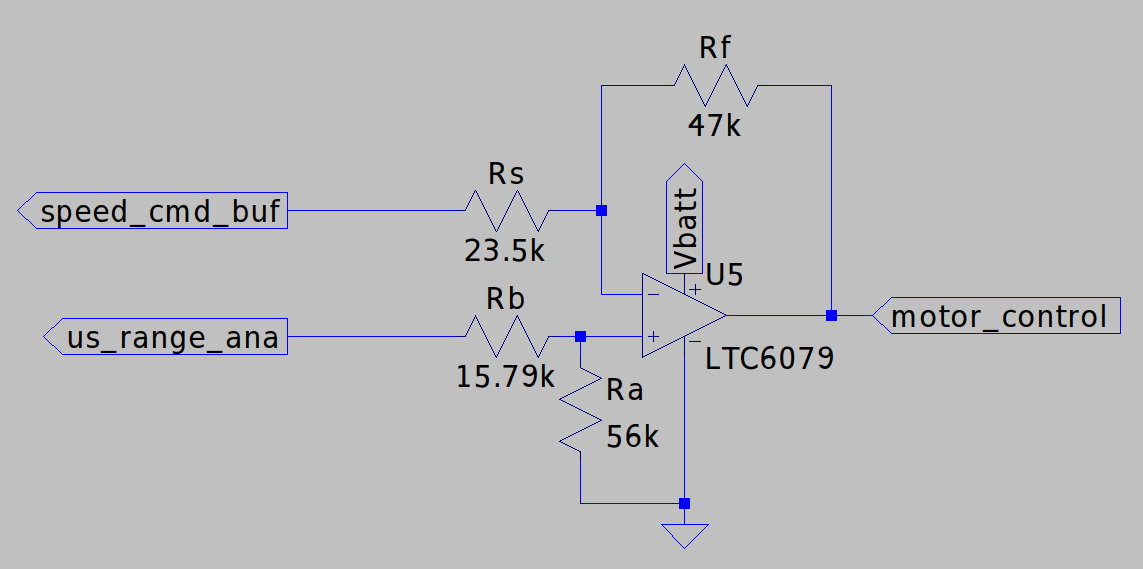
\includegraphics[width=1.0\linewidth]{motorController_subtractor_circuitDiagram}
        \captionof{figure}{Motor Controller Subtractor Stage Circuit Diagram}
        \label{fig:motorController_subtractor_circuitDiagram}
    \end{minipage}
    \begin{minipage}{.35\textwidth}
        \centering
        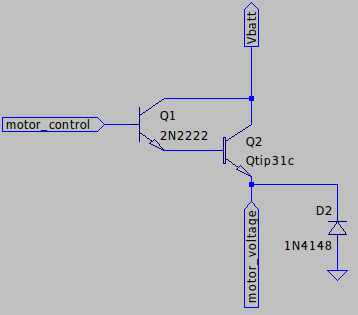
\includegraphics[width=1.0\linewidth]{motorController_power_circuitDiagram}
        \captionof{figure}{Motor Controller Power Stage Circuit Diagram}
        \label{fig:motorController_power_circuitDiagram}
    \end{minipage}
\end{figure}